%% Преамбула TeX-файла

% 1. Стиль и язык
\documentclass[utf8x]{G7-32} % Стиль (по умолчанию будет 14pt)
\usepackage[T2A]{fontenc}
\usepackage[russian]{babel}

% Остальные стандартные настройки убраны в preamble.inc.tex.
\sloppy

% Настройки стиля ГОСТ 7-32
% Для начала определяем, хотим мы или нет, чтобы рисунки и таблицы нумеровались в пределах раздела, или нам нужна сквозная нумерация.
\EqInChapter % формулы будут нумероваться в пределах раздела
\TableInChapter % таблицы будут нумероваться в пределах раздела
\PicInChapter % рисунки будут нумероваться в пределах раздела

% Добавляем гипертекстовое оглавление в PDF
\usepackage[
bookmarks=true, colorlinks=true, unicode=true,
urlcolor=black,linkcolor=black, anchorcolor=black,
citecolor=black, menucolor=black, filecolor=black,
]{hyperref}

% Изменение начертания шрифта --- после чего выглядит таймсоподобно.
% apt-get install scalable-cyrfonts-tex

\IfFileExists{cyrtimes.sty}
    {
        \usepackage{cyrtimespatched}
    }
    {
        % А если Times нету, то будет CM...
    }

\usepackage{graphicx}   % Пакет для включения рисунков

% С такими оно полями оно работает по-умолчанию:
% \RequirePackage[left=20mm,right=10mm,top=20mm,bottom=20mm,headsep=0pt]{geometry}
% Если вас тошнит от поля в 10мм --- увеличивайте до 20-ти, ну и про переплёт не забывайте:
\geometry{right=20mm}
\geometry{left=30mm}


% Пакет Tikz
\usepackage{tikz}
\usetikzlibrary{arrows,positioning,shadows}

% Произвольная нумерация списков.
\usepackage{enumerate}

% ячейки в несколько строчек
\usepackage{multirow}

% itemize внутри tabular
\usepackage{paralist,array}

\usepackage{natbib}

\bibliographystyle{apalike}
\bibpunct{[}{]}{,}{a}{}{;}

\usepackage{tabulary}
\usepackage{caption}



% Настройки листингов.
% 8 Листинги

\usepackage{listings}

% Значения по умолчанию
\lstset{
  basicstyle= \footnotesize,
  breakatwhitespace=true,% разрыв строк только на whitespacce
  breaklines=true,       % переносить длинные строки
%   captionpos=b,          % подписи снизу -- вроде не надо
  inputencoding=koi8-r,
  numbers=left,          % нумерация слева
  numberstyle=\footnotesize,
  showspaces=false,      % показывать пробелы подчеркиваниями -- идиотизм 70-х годов
  showstringspaces=false,
  showtabs=false,        % и табы тоже
  stepnumber=1,
  tabsize=4,              % кому нужны табы по 8 символов?
  frame=single
}

% Стиль для псевдокода: строчки обычно короткие, поэтому размер шрифта побольше
\lstdefinestyle{pseudocode}{
  basicstyle=\small,
  keywordstyle=\color{black}\bfseries\underbar,
  language=Pseudocode,
  numberstyle=\footnotesize,
  commentstyle=\footnotesize\it
}

% Стиль для обычного кода: маленький шрифт
\lstdefinestyle{realcode}{
  basicstyle=\scriptsize,
  numberstyle=\footnotesize
}

% Стиль для коротких кусков обычного кода: средний шрифт
\lstdefinestyle{simplecode}{
  basicstyle=\footnotesize,
  numberstyle=\footnotesize
}

% Стиль для BNF
\lstdefinestyle{grammar}{
  basicstyle=\footnotesize,
  numberstyle=\footnotesize,
  stringstyle=\bfseries\ttfamily,
  language=BNF
}

% Определим свой язык для написания псевдокодов на основе Python
\lstdefinelanguage[]{Pseudocode}[]{Python}{
  morekeywords={each,empty,wait,do},% ключевые слова добавлять сюда
  morecomment=[s]{\{}{\}},% комменты {а-ля Pascal} смотрятся нагляднее
  literate=% а сюда добавлять операторы, которые хотите отображать как мат. символы
    {->}{\ensuremath{$\rightarrow$}~}2%
    {<-}{\ensuremath{$\leftarrow$}~}2%
    {:=}{\ensuremath{$\leftarrow$}~}2%
    {<--}{\ensuremath{$\Longleftarrow$}~}2%
}[keywords,comments]

% Свой язык для задания грамматик в BNF
\lstdefinelanguage[]{BNF}[]{}{
  morekeywords={},
  morecomment=[s]{@}{@},
  morestring=[b]",%
  literate=%
    {->}{\ensuremath{$\rightarrow$}~}2%
    {*}{\ensuremath{$^*$}~}2%
    {+}{\ensuremath{$^+$}~}2%
    {|}{\ensuremath{$|$}~}2%
}[keywords,comments,strings]

% Подписи к листингам на русском языке.
\renewcommand\lstlistingname{\cyr\CYRL\cyri\cyrs\cyrt\cyri\cyrn\cyrg}
\renewcommand\lstlistlistingname{\cyr\CYRL\cyri\cyrs\cyrt\cyri\cyrn\cyrg\cyri}


% Полезные макросы листингов.
% Любимые команды
\newcommand{\Code}[1]{\textbf{#1}}


\begin{document}

\frontmatter % выключает нумерацию ВСЕГО; здесь начинаются ненумерованные главы: реферат, введение, глоссарий, сокращения и прочее.

% Команды \breakingbeforechapters и \nonbreakingbeforechapters
% управляют разрывом страницы перед главами.
% По-умолчанию страница разрывается.

% \nobreakingbeforechapters
% \breakingbeforechapters

% Также можно использовать \Referat, как в оригинале
\begin{abstract}
В данной работе исследована возможность использования се\-ман\-ти\-ко-син\-так\-си\-чес\-ко\-го
анализатора Compreno в качестве источника высокоуровневых признаков
для решения задачи распознавания именованных сущностей в рамках нейросетевого подхода.
Исследование проводилось на англоязычном корпусе CoNLL 2003.
Полученные результаты показывают, что высокоуровневые признаки
дают ощутимый прирост оценки качества, без какой-либо инженерии над ними.

\smallskip
\noindent \textbf{Ключевые слова:} нейронные сети, распознавание именованных сущностей.
\end{abstract}

%%% Local Variables:
%%% mode: latex
%%% TeX-master: "rpz"
%%% End:


\tableofcontents

\Introduction

  Именованная сущность - это слово или словосочетание обозначающее
  предмет или явления определенной категории. Примерами именованных сущностей
  являются имена людей, названия организаций и локаций.
  Задача распознавания именованных сущностей (Named Entity Recognition, NER)
  состоит в выделении и классификация именованных сущностей в тексте.
  В рамках конференции CoNLL 2003 проводилось соревнование
  для оценки качества методов распознавания именованных сущностей четырех типов
  на англоязычном корпусе \citep{tjong2003introduction}.
  Для решения задачи NER предлагалось много разных подходов \citep{nadeau2007survey}.
  В последнее время было показано, что методы на основе нейронных сетей показывают
  лучшие результаты для различных языков и корпусов, включая CoNLL 2003 \citep{DBLP:journals/corr/YangSC16}.

  Вместо большого количества вручную построенных признаков
  решающих определенную задачу, нейросетевые методы используют универсальные
  векторные представления слов \citep{mikolov2013distributed}.
  Согласно гипотезе о дистрибутивности, эти представления
  кодируют в себе смысл слов \citep{sahlgren2008distributional}.
  Это позволяет строить мультизадачные и языконезависимые
  архитектуры \citep{collobert2011natural, DBLP:journals/corr/YangSC16}.

  Несмотря на то, что использование универсальных векторных представлений
  получило в последнее время огромную популярность в силу своей эффективности
  и огромной экономии человеческих усилий, большой интерес все еще представляет
  исследование возможностей использования высокоуровневых признаков
  в качестве входных данных для нейросетей.
  Так, например, в работах \citep{xu2014rc, bian2014knowledge} описано использование
  морфологических, синтаксических и семантических признаков для построения
  более совершенных векторных представлений слов.

  Compreno -  это технология автоматического анализа текстов на естественном языке,
  в основе которой
  лежит многоуровневое лингвистическое описание, создававшееся профессиональными
  лингвистами в течение длительного времени \citep{anisimovich2012syntactic}.
  Помимо ручного описания Compreno использует для анализа большое количество
  информации, извлекаемых различными статистическими методами из текстовых корпусов.
  В Compreno реализована процедура семантико-синтаксического анализа текста,
  в результате которой любому предложению на естественном языке (английском или русском)
  ставится в соответствие семантико-синтаксическое дерево, моделирующее смысл предложения
  и содержащее грамматическую и семантическую информацию о каждом слове предложения.

  В данной работе исследована возможность использования семантико-синтаксического
  анализатора Compreno в качестве источника высокоуровневых признаков для задачи
  NER на корпусе CoNLL 2003 в рамках нейросетевого подхода.

  Статья организована следующим образом: в части 1 проведен обзор связанных работ.
  Выбранная нейросетевая модель и способы внедрения синтактико-семантических признаков описаны в части 2.
  В части 3 описаны проведенные эксперименты и программная реализация.

  Полученные результаты показывают повышение F1-меры почти на 1\% на корпусе CoNLL 2003
  при использовании синтактико-семантических признаков Compreno (87.49\% против 88.47\%).
  При этом затраты на их внедрение были минимальными - инженерия над признаками не проводилась.


\mainmatter % это включает нумерацию глав и секций в документе ниже

\chapter{Теоретико-аналитическая часть}

  \section{Постановка задачи}

    Исследовать возможность использования семантико-синтаксического
    анализатора Compreno в качестве источника высокоуровневых признаков для задачи
    NER на корпусе CoNLL 2003 в рамках нейросетевого подхода.

  \section{Обзор литературы}

    Победители соревнования по NER CoNLL 2003 \citep{florian2003named}, получившие 88.76\% F1,
    представили систему использующую комбинацию различных алгоритмов машинного обучения.
    В качестве признаков был использован их собственный, вручную составленный газетир,
    POS-теги, CHUNK-теги, суффиксы, префиксы и выход других NER-классификаторов,
    тренированных на внешних данных.

    \citep{collobert2011natural} представили комбинацию сверточной нейронной сети
    с условными случайными полями, получившую 89.59\% F1 на корпусе CoNLL 2003.
    Их нейросетевая архитектура не зависит от задачи и используется как для NER, так и для
    частеречной разметки (part-of-speech tagging), поиска синтаксически связанных групп
    соседних слов (chunking), установления семантических ролей (semantic role labelling).
    Для задачи NER они использовали три типа признаков - векторное представление слова,
    капитализацию и небольшой газетир, включенный в соревнование CoNLL 2003.

    \citep{chiu2015named} представили комбинацию сверточных сетей, рекуррентных сетей
    и условных случайных полей показывающую 91.62\% F1.
    Они использовали такие же признаки как у \citep{collobert2011natural}, дополнительный, вручную сформированный
    газетир на основе DBpedia и обучались на
    train+dev\footnote{Объединенная обучающая и валидационная выборки} выборке CoNLL 2003.
    Кроме корпуса CoNLL 2003 они тестировали архитектуру
    на более крупном англоязычном корпусе OntoNotes 5.0. На нем они получили
    state-of-the-art результат 86.28\%.

    \citep{DBLP:journals/corr/YangSC16} представили глубокую иерархическую рекуррентную нейросетевую
    архитектуру с условными случайными полями для разметки последовательностей.
    Они использовали такие же признаки как у \citep{collobert2011natural}.
    Кроме англоязычного корпуса CoNLL 2003, где они получили state-of-the-art 90.94\% F1 при обучении
    только на обучающей выборке (train set), они тестировали работу нейросети на CoNLL 2002 Dutch NER и CoNLL 2003 Spanish NER.
    На этих корпусах они улучшили предыдущий state-of-the-art результат:
    82.82\% до 85.19\% на CoNLL 2002 Dutch NER и 85.75\% до 85.77\% на CoNLL 2003 Spanish NER.

    Современные работы используют векторное представление слов
    и условные случайные поля в своих моделях. Из сторонних признаков применяют
    только газетиры. В работах \citep{xu2014rc, bian2014knowledge} описано применение дополнительных признаков для
    слов (морфологических, синтаксических, семантических) для создания более
    совершенных векторных представлений.
    Такие векторные представления помогают повысить оценку качества в
    прикладных задачах \citep{xu2014rc}.

  \section{Обзор корпуса CoNLL 2003}

  В данной работе рассмотрен англоязычный корпус CoNLL 2003, т.к. он является
  одним из самых распространенных корпусов на котором год от года измеряют оценку качества
  методов распознавания именованных сущностей.

  CoNLL 2003 \citep{tjong2003introduction} - англоязычный корпус для оценки качества
  методов распознавания именованных сущностей.
  Корпус содержит обучающую, тестовую и валидационную выборку.
  Размечено 4 типа сущностей - персоны (PER), организации (ORG), локации (LOC) и другие (MISC).
  \newpage
  \begin{table}[!h]
    \caption{Количество статей, предложений, токенов и именованных сущностей}
    \centering
    \begin{tabular}{ | p{2.9cm} | p{1.5cm} | p{2.5cm} | p{1.5cm} | p{1cm} | p{1.1cm} | p{1cm}| p{1cm} |}
      \hline\hline
      Выборка & Статьи & Предлож-я & Токены & LOC & MISC & ORG & PER \\
      \hline
      Обучающая & 946 & 14987 & 203621 & 7140 & 3438 & 6321 & 6600 \\
      \hline
      Валидац-я & 216 & 3466 & 51362 & 1837 & 922 & 1341 & 1842 \\
      \hline
      Тестовая & 231 & 3684 & 46435 & 1668 & 702 & 1661 & 1617 \\
      \hline
    \end{tabular}
  \end{table}

  Корпус размечен по схеме \textit{Inside, Outside, Begin (IOB)}:
  \begin{itemize}
  \item слово помечают тегом O (Outside), если оно не является именованной сущностью.
  \item Тегом I-XXX (Inside), где XXX - тип именованной сущности, если слово
    является именованной сущности или ее частью.
  \item Тегом B-XXX (Begin), если слово является началом именованной сущности.
  \end{itemize}

  Пример:
  \centerline{}
  \centerline{, O}
  \centerline{Surrey I-ORG}
  \centerline{captain O}
  \centerline{Chris B-PER}
  \centerline{Lewis I-PER}
  \centerline{, O}

  Оценка качества считается с помощью метрики $F_{\beta=1}$(F1-micro-average):
  \[
    F_\beta = \frac{(\beta^2 + 1) * precision * recall}{\beta^2*precision + recall},
  \]
  где $precision$ (точность) - процент корректных именованных сущностей
  найденных системой, $recall$ (полнота) - процент всех именованных сущностей
  найденных системой. Именованная сущность считается найденной корректно, если
  вся сущность помечена правильно.
  В CoNLL 2003 включен скрипт conlleval, оценивающий качество классификации.

  В работе \citep{collobert2011natural} предлагается использовать схему
  \textit{Inside, Outside, Begin, End, Single (IOBES)}, т.к. она более явно указывает
  тег для слова:
  \begin{itemize}
  \item слово помечают тегом O (Outside), если оно не является именованной сущностью.
  \item Тегом I-XXX (Inside), где XXX - тип именованной сущности, если слово является частью именованной сущности.
  \item Тегом B-XXX (Begin), если слово является началом именованной сущности.
  \item Тегом E-XXX (End), если слово является концом именованной сущности.
  \item Тегом S-XXX (Single), если именованная сущность состоит из одного слова.
  \end{itemize}

  Пример:
  \centerline{}
  \centerline{, O}
  \centerline{Surrey S-ORG}
  \centerline{captain O}
  \centerline{Chris B-PER}
  \centerline{Lewis E-PER}
  \centerline{, O}

  Во время оценки качества, IOBES конвертируют в IOB и подают на вход conlleval.

  Также в CoNLL 2003 включен небольшой газетир.

  \section{Обзор нейросетевого подхода к решению задачи NER}  \label{section:nn}

  Традиционным подходом к решению задач из области автоматической обработки текстов,
  включая NER, является использованием алгоритма обучения с учителем, например
  машины опорных векторов с линейным ядром. Вручную составленные признаки подаются на вход
  алгоритма обучения с учителем. Выбор признаков - это практически полностью эмпирический
  процесс, построенный на лингвистической интуиции и решаемой задаче.

  Нейросетевой подход предполагает использование минимального количества признаков.
  Обычно это векторные представления слов полученные из большого корпуса с использованием
  алгоритмов обучения без учителя.

  В этом разделе будет рассмотрен нейросетевой подход из работы
  \citep{collobert2011natural}. Была выбрана именно эта работа так как:
  \begin{itemize}
  \item в ней представлена модель, получающая сравнимую со state-of-the-art F1-меру на CoNLL 2003,
  \item представленная модель имеет различные программные имплементации,
  \item векторные представления слов под названием <<Senna Embeddings>>
    используемые в этой работе находятся в открытом доступе в сети.
  \end{itemize}
  Последние два пункта указывают на возможность воспроизведения результатов из статьи относительно небольшими усилиями.

  \subsection{Векторные представления слов}

  Согласно Википедии\footnote{\url{https://en.wikipedia.org/wiki/Word_embedding}},
  \textit{векторное представление} — это общее название для различных
  подходов к моделированию языка и обучению представлений в обработке естественного языка,
  направленных на сопоставление словам (и, возможно, фразам) из некоторого словаря $D$,
  векторов из $R^n$, где $n$ - значительно меньше $|D|$ (обычно от 50 до 1000).

  \citep{collobert2011natural} использовали нейронные сети для построения векторных представлений слов.
  Они тренировали нейронную сеть на данных корпуса английской
  Википедии\footnote{На данных ноября 2007 года из http://download.wikimedia.org}
  и Reuters RCV1\footnote{Доступно http://trec.nist.gov/data/reuters/reuters.html}.
  Были использованы 130000 самых частотных слов, остальные слова кодировались
  специальным токеном UNKNOWN.
  Полученные векторные представления называются Senna Embeddings и доступны в сети
  по адресу: http://ronan.collobert.com/senna/.

  Senna Embeddings использовались как входные признаки на нейронные сети для решения задачи NER.

  \subsection{Описание нейросетевых моделей} \label{subsection:nn}

  В работе \citep{collobert2011natural} описываются две нейросетевые модели:
  \begin{itemize}
  \item оконный (window), который предсказывает тег слова на основе контекста (окна) вокруг слова,
  \item сверточный (convolution), который предсказывает тег слова используя всё предложение.
  \end{itemize}

  \subsubsection{Оконная модель} \label{subsubsection:window}
  Оконная модель представлена на рис. \ref{figure:window_net}.
  \newpage
  \begin{figure}[!h]
    \centering
    \caption{Оконная модель из \citep{collobert2011natural}}
    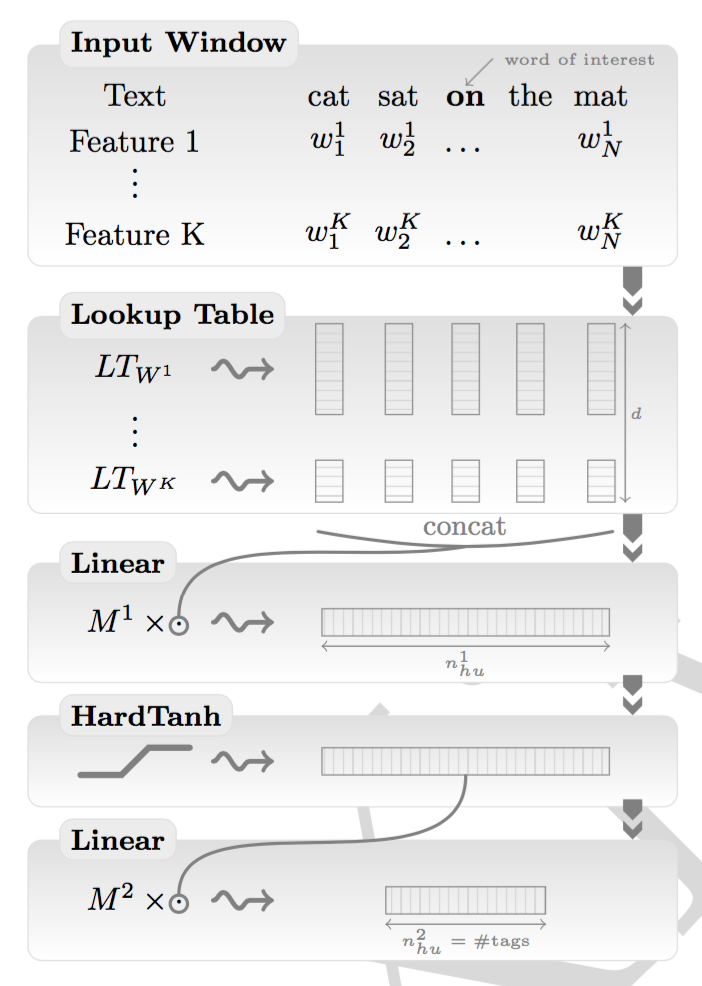
\includegraphics{figures/window.png}
    \label{figure:window_net}
  \end{figure}

  На рис. \ref{figure:window_net} предсказывается тег для слова on.
  При классификации используется контекст для этого слова.
  Всё окно состоящее из 5 слов пропускается через так называемый Lookup Table.

  \textit{Lookup Table} - это специальной слой в нейронной сети, который
  отображает каждое слово в вектор весов. Причем вектор весов обучается вместе с сетью.
  Более формально, каждому слову $w$ из словаря $D$ ставится в соответствие
  вектор размерности $d$, который задается Lookup Table слоем $LT_W(w)$:
  \[
    LT_W(w) = W_{\cdot,w},
  \]
  где $W \in R^{d\times|D|}$ - матрица весов для обучения, $W_{\cdot,w}$ - $w$-ый столбец
  матрицы $W$. Размерность $d$ - гиперпараметр.

  Также этот слой может принимать на вход последовательность слов $w_1 \ldots w_K$,
  где $K$ - величина окна. В этом случае выходом будет матрица:
  \[
    f_1 = LT_W(w_1 \ldots w_K) = ( W_{\cdot, w_1} \ldots W_{\cdot, w_K})
  \]

  После Lookup Table слоя, полученная матрица преобразуется в один вектор с
  помощью операции \textit{конкатенации (Concat)}:
  \[
    f_{2} = Concat(LT_W(w_1 \ldots w_K)) =
      \begin{bmatrix}
        W_{\cdot, w_1} \\
        \vdots \\
        W_{\cdot, w_K}
      \end{bmatrix},
  \]

  Затем этот вектор подается на \textit{полносвязный слой (Linear Layer)}, который
  выполняет аффинное преобразование:
  \begin{equation} \label{formula:linear_layer}
    f_{3} = Linear(f_{2}) = W^2 f_{2} + b^2,
  \end{equation}
  где $W^2 \in R^{d_{2} \times |f_{2}|}$, $b \in R^{d_2}$. Гиперпараметр $d_{2}$ -
  это количество нейронов в данном слое.

  Каждый элемент полученного вектора $f_3 \in R^{d_2}$ пропускается через нелинейную функцию.
  На рис. \ref{figure:window_net} это \textit{HardTanh}:
  \[
    f_{4} = HardTanh(f_{3}),
  \]
  \begin{equation} \label{formula:hard_tanh}
  HardTanh(x) =
    \begin{cases}
      -1, \text{if } x < -1 \\
      x, \text{if } -1 <= x <= 1 \\
      1, \text{if } x > 1
    \end{cases}
  \end{equation}
  Преимуществом этой функции перед гиперболическим тангенсом является более быстрое
  время вычисления.

  Последний слоем является полносвязный слой. Количество нейронов в нем
  равно количеству предсказываемых классов.
  \[
    f_5 = Linear(f_4) = W^5 f_{4} + b^5.
  \]

  Каждый элемент $x_i$ полученного вектора $f_5$ пропускается через функцию \textit{Softmax} для получения
  вероятностей:
  \[
    Softmax(x_{i}) = \frac{e^{x_{i}}}{\sum_j e^{x_{j}}}
  \]
  Другими словами это нормализация вектора с помощью экспоненциальной функции.

  Для обучения нейронной сети минимизируется функционал ошибки с использованием
  пакетного градиентного спуска (mini-batch gradient descent).
  \textit{Функционал ошибки $C$}:
  \[
    C = - \sum_{(x, y_k) \in T} \log(\Prob(y_k | x, \theta)),
  \]
  \[
    C \rightarrow \min_\theta,
  \]
  \[
    \log(\Prob(y_k | x, \theta)) = f_4(y_k) - \log\sum_i e^{f_4(y_i)},
  \]
  где $(x, y_k)$ - пара объект, класс из обучающей выборки $T$; $\theta$ - веса
  всей нейросети (все матрицы $W$), $f_4(y_i)$ - значение последнего слоя для класса $y_i$.

  Функционал ошибки $C$ минимизируется с помощью \textit{пакетного градиентного спуска}:
  \[
    \theta = \theta - \alpha\sum_{(x, y_k) \in T_s}\nabla_{\theta}(-\log\Prob(y_k | x, \theta)),
  \]
  где $\alpha$ - шаг обучения, $T_s$ - случайное подмножество объектов из обучающей выборки.
  Размер подмножества $T_s$ и $\alpha$ являются гиперпараметрами.

  \textit{Стохастический градиентный спуск (stochastic gradient descent)} является
  модификацией пакетного градиентного спуска. Отличие заключается в том, что размер $T_s$ равен 1.

  \subsubsection{Сверточная модель}  \label{subsubsection:conv}
  Сверточная модель представлена на рис. \ref{figure:conv_net}.
  \newpage
  \begin{figure}[!h]
    \centering
    \caption{Сверточная модель из \citep{collobert2011natural}}
    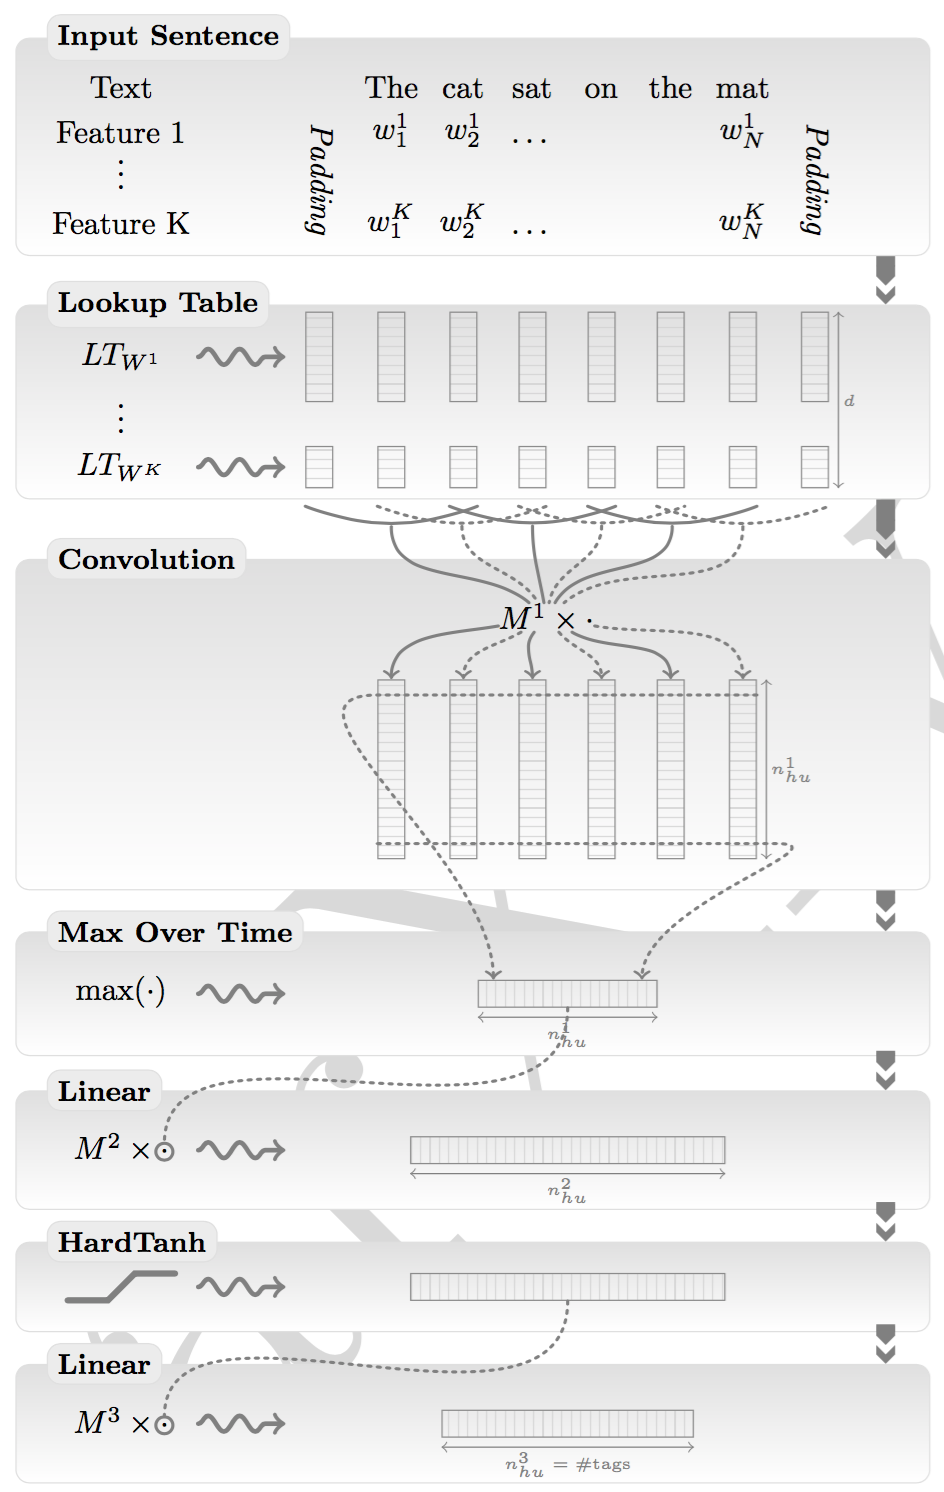
\includegraphics[scale=0.9]{figures/sentence-diagram.png}
    \label{figure:conv_net}
  \end{figure}

  В отличие от оконной модели, она принимает на вход всё предложение.

  Все слова предложения пропускаются через Lookup Table, как описано в разделе
  \ref{subsubsection:window}, после чего попадают на сверточный слой.

  \textit{Сверточный слой (temporal convolution)} является обобщением
  полносвязного слоя (\ref{formula:linear_layer}) из оконного подхода:
  \begin{enumerate}
    \item сначала осуществляется проход окном на полученной на предыдущем шаге матрице $f_1$,
    \item столбцы попавшие в окно конкатенируются,
    \item полученный вектор пропускается через полносвязный слой,
    причем матрица весов $W^3$ является одной и той же в каждом проходе.
  \end{enumerate}
  На выходе, после прохода окном по всей матрице $f_1$, получается матрица $f_3$.
  Более формально:
  \[
  f_3 =(W^3 f_1[1, d_{win}] + b^3,\ldots,W^3 f_1[|f_1| - d_{win}, d_{win}] + b^3),
  \]
  \[
  d_{f_1, win} = d_{win}*d,
  \]
  где $f_1[i, d_{win}]$ - означает конкатенацию столбцов $f_1$ с $i$ по $i + d_{win}$,
  $d_{f_1, win}$ - размерность полученного после конкатенации вектора $f_1[i, d_{win}]$,
  $W^3 \in R^{d_{2} \times d_{f_1, win}}$, $b \in R^{d_2}$. Гиперпараметр $d_{2}$ -
  это количество нейронов в данном слое.

  После того как всё предложение прошло через Lookup Table и сверточный слой
  получается матрица $f_3 \in R^{d_2\times |f_1| - d_{win}}$.
  Количество строк в ней фиксировано, но количество столбцов зависит от длины предложения.
  Чтобы получить вектор признаков фиксированный длины выполняется \textit{операция
  получения максимума по строкам (Max over time)} над $f_3$.
  Смысл этой операции заключается в получении наиболее значимых признаков из каждого окна.
  Из каждой строки матрицы $f_3$ извлекается максимум и в результате этой
  операции получается вектор $f_5 \in R^{d_2}$.

  Далее над полученным фиксированным вектором признаков проводятся уже
  знакомые по разделу \ref{subsubsection:window}
  операции с полносвязными слоями (\ref{formula:linear_layer}) и
  нелинейной функцией HardTanh (\ref{formula:hard_tanh}).

  Для обучения используется минимизация функционала ошибки и пакетный градиентный
  спуск описанные в разделе \ref{subsubsection:window}.

  В оригинальное статье \citep{collobert2011natural} в сверточном подходе
  минимизировался другой функционал ошибки, который включает в себя условные случайные поля.
  Это позволило им достичь более высокой оценки качества, но в то же время замедлило
  время проведения экспериментов. Данный функционал не поддерживается библиотеками для
  работы с нейронными сетями, поэтому его необходимо реализовывать с нуля.
  Из-за этих причин этот функционал ошибки не рассмотрен в этой работе.

  \subsubsection{Уточнения к моделям}

  В разделе \ref{subsubsection:conv} теги предсказываются для каждого слова.
  Т.к. на вход нейросети поступает предложение, то необходимо кодировать
  местоположение слова в предложении для которого предсказывается тег.
  Это осуществлялось с помощью Lookup Table.
  Позиция слова $w_j$ в предложении кодировалась
  с помощью подсчета расстояния относительно слова $w_i$ для которого предсказывается тег.
  Слово $w_i$ кодировалось в Lookup Table как $0$. Слово $w_{i-k}$ как $-k$. Слово $w_{i+k}$ как $+k$.

  В качестве регуляризации использовался Dropout слой после каждого полносвязного слоя,
  кроме последнего.
  Dropout слой \citep{srivastava2014dropout} с заданной вероятностью $p$ зануляет
  выход нейрона.

  Важным условием хорошего обучения нейронной сети является начальная инициализация
  весов. В данной работе использовано 2 подхода к инициализации весов:
  \begin{enumerate}
  \item $U(\frac{-1}{\sqrt{fi}}, \frac{1}{\sqrt{fi}})$
  \item $U(-\sqrt{\frac{2}{fi + fo}}, \sqrt{\frac{2}{fi + fo}}),$
  \end{enumerate}
  где $U$ - равномерное распределение, $fi$ - количество входов в слой,
  $fo$ - количество выходов из слоя.
  Первый подход описан в \citep{collobert2011natural}, второй в \citep{glorot2010understanding}.


  \section{Обзор синтактико-семантических признаков}
    Существует много инструментов для получения дополнительных признаков для слова.
    Для извлечения синтаксических признаков часто используют MaltParser \citep{nivre2006maltparser}.
    Для получения семантических признаков применяют BabelNet \citep{navigli2010babelnet}.

    В данной работе для получения синтактико-семантических признаков используется Compreno.
    Признаки синтактико-семантического дерева Compreno кодировались в бинарные вектора
    и соотносились с токенами исходного
    текста\footnote{Почти для всех токенов в соответствующем дереве нашлась соответствующая вершина.
    Токены для которых не была найдена вершина, кодировались специальным признаком 83951},
    тем самым наделяя их синтактико-се\-ман\-ти\-ческими признаками.
    Размерность пространства синтактико-се\-ман\-ти\-ческих признаков получилась равной 83951.

    Плотные вектора большой размерности сильно замедляют процесс оптимизации и для хорошего
    обучения требуется много данных и вычислительных ресурсов.
    В таких случаях часто применяют методы для уменьшения размерности,
    например сингулярное разложение (SVD) или автоэнкодеры. Минусом таких методов является потеря информации
    после сжатия.

    Если же вектора большой размерности разреженные, то используют специальные методы для
    работы с такими данными \citep{davissurvey}.

    В данной работе предлагается 2 способа внедрения синтактико-семантических признаков:
    \begin{itemize}
      \item сжать синтактико-семантические вектора с помощью сингулярного разложения и добавить
      как еще один Lookup Table в сверточную нейронную сеть;
      \item добавить еще одну нейронную сеть для синтактико-семантических признаков и оптимизировать
      её вместе со сверточной нейронной сетью.
    \end{itemize}


\chapter{Проектная часть}

\section{Описание моделей} \label{section:models}

Для экспериментов были реализованы следующие модели:
\begin{itemize}
\item оконная (WindowNet) - данная модель подробно описана в разделе \ref{subsubsection:window},
\item сверточная (ConvNet) - данная модель подробно описана в разделе \ref{subsubsection:conv},
\item полносвязная нейронная сеть для работы с разреженными синтактико-семантическими признаками (ComprenoNet),
\item комбинация сверточной и полносвязной сети (ConvNet + ComprenoNet)
\end{itemize}

\subsection{Гиперпараметры моделей и признаки}

Общие для всех моделей гиперпараметры:
\begin{itemize}
\item $\alpha=0.01$ - шаг обучения,
\item $p=0.5$ - вероятность для Dropout слоя,
\item количество нейронов в последнем полносвязном слое равно 17,
т.к. используется схема IOBES. Четыре для каждого из четырех типов тегов и один для Outside.
\end{itemize}

Гиперпараметры для оконной модели (рис. \ref{figure:window_net}) следующие:
\begin{itemize}
\item $d_2 = 300$ - количество нейронов в полносвязном слое,
\item $K=5$ - величина окна. Если в окне нет слов, то окно дополняется специальным токеном PADDING,
\item $|T_s|=32$ - размер подмножества для пакетного градиентного спуска.
\end{itemize}

Гиперпараметры для сверточной модели (рис. \ref{figure:conv_net}) следующие:
\begin{itemize}
\item $d_2 = 300$ - количество нейронов в сверточном слое,
\item количество нейронов в полносвязном слое также равно 300,
\item $d_{win} = 3$ - величина окна. Если в окне нет слов, то окно дополняется специальным токеном PADDING,
\item $|T_s|=33$ - размер подмножества для пакетного градиентного спуска.
\end{itemize}

Для экспериментов были использованы следующие признаки:
\begin{itemize}
\item Embeddings - векторные представления слов Senna Embeddings,
\item Capitalization - дискретный признак капитализации слова с 5 возможными вариантами
(слово начинается с большой буквы, слово содержит большую букву,
все символы в слове состоят из больших букв, нет больших букв в слове, не слово),
\item Position - кодирование позиции слова в предложении (описано в разделе \ref{subsubsection:conv}),
\item Gazetteer - проверяется присутствие слова в газетире CoNLL 2003,
\item Compreno sparse features - синтактико-се\-ман\-ти\-ческие признаки Compreno размерности 83951,
\item Compreno SVD 1024 - синтактико-семантически признаки Compreno размерности 83951 были сжаты с использованием
модификации сингулярного разложения для работы с разреженными признаками
TruncatedSVD\footnote{http://scikit-learn.org/stable/modules/generated/sklearn.decomposition.TruncatedSVD.html}
до размерности 1024. После сжатия описываемая дисперсия была равна 72\%. Т.е. потерялось 28\% информации.
\end{itemize}

Все признаки, кроме Compreno sparse features, были включены в нейронные сети с использованием Lookup Table.


\subsection{ComprenoNet}

Архитектура и гиперпараметры полносвязной нейронной сети для работы с разреженными
синтактико-семантическими признаками (ComprenoNet) представлены ниже:
\begin{lstlisting}
input -> (1) -> (2) -> (3) -> (4) -> (5) -> (6) -> (7) -> output
(1): nn.SparseLinear(83951, 256)
(2): nn.Dropout(0.5)
(3): nn.HardTanh
(4): nn.Linear(256 -> 256)
(5): nn.Dropout(0.5)
(6): nn.HardTanh
(7): nn.Linear(256 -> 17)
\end{lstlisting}

SparseLinear представляет из себя обычный полносвязный слой (Linear), который
оптимизирован для работы с разреженными данными. Другие слои и процесс обучения
аналогичны тем, что были описаны в разделе \ref{subsection:nn}.
Общий алгоритм работы сети следующий:
\begin{enumerate}
  \item на вход подается разреженный вектор признаков слова (размерность 83951) для которого предсказывается тег.
  \item Далее этот вектор пропускается через 2 полносвязных слоя.
  \item На выходе еще один полносвязный слой, который выдает вероятность определенного тега.
  Выходов также 17.
\end{enumerate}

\subsection{ConvNet + ComprenoNet}

Архитектура и гиперпараметры комбинации сверточной и полносвязной сети (ConvNet + ComprenoNet)
представлены на рис. \ref{figure:two_net}.
\begin{figure}[!h]
  \centering
  \caption{Комбинация сверточной и полносвязной сети (ConvNet + ComprenoNet)}
  \includegraphics[scale=0.5]{figures/two-net.png}
  \label{figure:two_net}
\end{figure}
Эти сети соединяются следующим образом:
\begin{enumerate}
  \item Из обеих нейросетей удаляются выходные слои.
  \item Предыдущие слои из обеих сетей соединяются в новый полносвязный слой.
  \item Новый полносвязный слой соединяется с выходным слоем. Выходов как и тегов 17.
\end{enumerate}
Веса у объединенной сети были инициализированы предобученными моделями (ConvNet, ComprenoNet).
Слои нейронной сети и процесс обучения аналогичны тем, что были описаны в разделе \ref{subsection:nn}.

\section{Программная реализация}

Для программной реализации описанных выше моделей существуют различные фреймворки
для нейронных сетей.
\textit{Фреймворк}, согласно Википедии\footnote{\url{https://en.wikipedia.org/wiki/Software_framework}} - это
программная платформа, определяющая структуру программной системы; программное обеспечение,
облегчающее разработку и объединение разных компонентов большого программного проекта.

Выбору фреймворка для работы с нейросетями посвящена работа \citep{bahrampour2015comparative}.
В ней они сравнивали такие программные платформы как:
\begin{itemize}
\item Caffe,
\item Neon,
\item TensorFlow,
\item Theano,
\item Torch.
\end{itemize}
В таблице \ref{table:framework_comparison} из \citep{bahrampour2015comparative}
указаны особенности этих фреймворков.

\begin{table}[!h]
  \caption{Особенности нейросетевых фреймворков}
  \centering
  \begin{tabulary}{\textwidth}{| L | L | L | L | L | L | L |}
    \hline\hline
    \multicolumn{1}{|p{1.7cm}|}{Фреймворк} & Caffe & Neon & TensorFlow & Theano & Torch \\
    \hline
    Язык & C++ & Python & C++ & Python & Lua \\
    \hline
    CPU & + & + & + & + & + \\
    \hline
    Поддержка многопоточ-и CPU & + & - & + & + & + \\
    \hline
    GPU & + & + & + & + & + \\
    \hline
    Поддержка неск-х GPU & + & + & + & - & + \\
    \hline
    Nvidia cuDNN & + & - & + & + & + \\
    \hline
    Простота модификации & - & - & +- & + & + \\
    \hline
    Поддержка сообществом & +++ & + & ++ & +++ & ++ \\
    \hline
  \end{tabulary}
  \label{table:framework_comparison}
\end{table}

Практически все современные нейросетевые библиотеки поддерживают работу
с графическими процессорами (GPU).
Производители GPU делают специальные библиотеки для научных
вычислений на графических процессорах.
Например, Nvidia cuDNN (NVIDIA CUDA Deep Neural Network library) -
библиотека, которая ускоряет вычисления для нейронных сетей.
Использование графических процессоров позволяет ускорить обучение нейросетей
в разы по сравнению с центральным процессорным устройством (CPU).
Некоторые фреймворки поддерживают работу с несколькими GPU одновременно для
еще более быстрой работы нейросетей.

Есть программные платформы заточенные для решения одной определенной задачи.
Например, Caffe - нейросетевой фреймворк для решения задач связанных с компьютерным зрением.
Его использование для текстовых данных является затруднительным.
В то же время есть универсальные фреймворки, такие как Torch, TensorFlow,
которые позволяют решать задачи с использование нейронных сетей в различных
областях, включая автоматическую обработку текстов.
Они имеют гибкую архитектуру, поэтому их можно достаточно просто модифицировать.

Все фреймворки описанные в таблице \ref{table:framework_comparison} являются
общедоступными, имеют открытый код и поддерживаются сообществом разработчиков и
разными компаниями. Например, TensorFlow поддерживает компания Google, torch
компания Facebook.

Также стоит отметить, что сверточная модель описанная в разделе \ref{subsubsection:conv}
уже имеет программную реализацию в открытом доступе в сети по адресу: http://ronan.collobert.com/senna/.
Минусом данной реализации является то, что она написана без использования
нейросетевых фреймворков, на языке программирования C, не поддерживает GPU,
не поддерживается сообществом, имеет тяжелый в понимании код, заточена под конкретную задачу
и не содержит в себе различные современные нейросетевые решения, например Dropout.

Исходя из следующих требований:
\begin{itemize}
\item гибкость в реализации нейросетевых архитектур,
\item быстрота проведения экспериментов,
\item поддерживаемый код,
\end{itemize}
был выбран нейросетевей фреймворк torch\footnote{\url{http://torch.ch}}.

Код для воспроизведения экспериментов выложен по адресу:
\href{https://github.com/sld/torch-conv-ner}{github.com/sld/torch-conv-ner}.

Скорость обучения на машине с GPU Amazon AWS g2.2xlarge\footnote{https://aws.amazon.com/ru/ec2/instance-types/}:
\begin{itemize}
\item 1 эпоха\footnote{Эпоха - это один полный проход по обучающей выборке} при одиночной обработке (stochastic gradient descent): $\sim$450 сек.
\item 1 эпоха при пакетной обработке (mini-batch gradient descent): $\sim$171 сек.
\item Модель получающая 87.49\% обучалась 91 эпоху ($\sim$4.2 часа).
\item 1 эпоха при пакетной обработке с использованием признаков Compreno: $\sim$615 сек.
\end{itemize}

Скорость классификации составляет 2500 токенов в секунду при пакетной обработке.

\newpage

\section{Эксперименты}

\subsection{Эксперименты без синтактико-семантических признаков}
По таблице \ref{table:raw_net} видно, что результаты немного ниже чем у \citep{collobert2011natural}.
Это связано с тем, что для Window подхода использован другой метод оптимизации,
а для Convolution подхода не были применены условные случайные поля (ConvNet + CRF в таблице \ref{table:raw_net}).

В качестве референсной, будет использована модель из последнего эксперимента
показывающая 87.49\% F1.
Это сделано для чистоты эксперимента, т.к. далее  обучение происходило только
на обучающей выборке по правилам соревнования CoNLL 2003 и применялся пакетный
градиентный спуск для ускорения экспериментов.

\newpage

\begin{table}[!h]
  \caption{Результаты экспериментов без использования синтактико-семантических признаков}
  \centering
  \begin{tabulary}{\textwidth}{| L | L | L | L | L | L |}
    \hline\hline
    \multicolumn{1}{|p{1.7cm}|}{Модель} & Признаки & Выборка & Метод оптимизации & Полученная F1, \% & F1 в статье \cite{collobert2011natural} \\
    \hline
    Window & Embeddings, Capitalization & train & Mini-batch gradient descent & 86.27 & - \\
    \hline
    Window & Embeddings, Capitalization & train & Stochastic gradient descent & - & 86.97 \\
    \hline
    ConvNet + CRF & Embeddings, Capitalization, Position & train & Stochastic gradient descent & - & 88.67 \\
    \hline
    ConvNet + CRF & Embeddings, Capitalization, Position, Gazetteer & train & Stochastic gradient descent & - & 89.59 \\
    \hline
    ConvNet & Embeddings, Capitalization, Position & train & Stochastic gradient descent & 86.77 & - \\
    \hline
    ConvNet & Embeddings, Capitalization, Position, Gazetteer & train & Stochastic gradient descent & 87.89 & - \\
    \hline
    ConvNet & Embeddings, Capitalization, Position, Gazetteer & train + dev & Stochastic gradient descent & 88.37 & - \\
    \hline
    ConvNet & Embeddings, Capitalization, Position, Gazetteer & train & Mini-batch gradient descent & \textbf{87.49} & - \\
    \hline
  \end{tabulary}
  \label{table:raw_net}
\end{table}

\subsection{Эксперименты с синтактико-семантическими признаками сжатыми с использованием SVD}

\begin{table}[!h]
  \caption{Результаты с синтактико-семантическими признаками сжатыми SVD}
  \centering
  \begin{tabulary}{\textwidth}{| L | L | L | L | L | L |}
    \hline\hline
    \multicolumn{1}{|p{1.7cm}|}{Модель} & Признаки & Выборка & Метод оптимизации & Полученная F1, \% \\
    \hline
    ConvNet & Position, Compreno SVD 1024 & train & Mini-batch gradient descent & 75.89 \\
    \hline
    ConvNet & Capitalization, Position, Gazetteer, Compreno SVD 1024 & train & Mini-batch gradient descent & 81.83 \\
    \hline
    ConvNet & Embeddings, Capitalization, Position, Gazetteer, Compreno SVD 1024 & train & Mini-batch gradient descent & 86.85 \\
    \hline
    ConvNet & Embeddings, Capitalization, Position, Gazetteer & train & Mini-batch gradient descent & 87.49 \\
    \hline
  \end{tabulary}
  \label{table:svd_net}
\end{table}


По таблице \ref{table:svd_net} видно, что такой способ ведет к небольшому ухудшению F1-меры.
Это может быть связно с тем, что после применения сингулярного разложения
было потеряно 28\% информации о синтактико-семантических признаках Compreno.


\subsection{Эксперименты с синтактико-семантическими признаками на ConvNet + ComprenoNet}

Веса у ConvNet + Compreno Net были инициализированы обученными моделями -
моделью показывающую 87.49\% для сверточной сети и моделью показывающую
72.85\% (см. таблицу \ref{table:union_net}) для второй нейронной сети.

\begin{table}[ht]
  \caption{Результаты с синтактико-семантическими признаками для объединенной нейросети}
  \centering
  \begin{tabulary}{\textwidth}{| L | L | L | L | L | L |}
    \hline\hline
    \multicolumn{1}{|p{1.5cm}|}{Модель} & Признаки & Выборка & Метод оптимизации & Полученная F1, \% \\
    \hline
    Compreno Net & Compreno sparse features & train & Mini-batch gradient descent & 72.85 \\
    \hline
    ConvNet & Embeddings, Capitalization, Position, Gazetteer & train & Mini-batch gradient descent & 87.49 \\
    \hline
    ConvNet + Compreno Net & Embeddings, Capitalization, Position, Gazetteer, Compreno sparse features & train & Mini-batch gradient descent & \textbf{88.47} \\
    \hline
    ConvNet + Compreno Net & Embeddings, Capitalization, Position, Gazetteer, Compreno sparse features & train + dev & Mini-batch gradient descent & 88.81 \\
    \hline
  \end{tabulary}
  \label{table:union_net}
\end{table}

По таблице \ref{table:union_net} видно, что в этом случае признаки Compreno
улучшают F1-меру почти на один процент.


% \chapter{Экспериментальная часть}

\section{Корпус CoNLL 2003}

CoNLL 2003 \citep{tjong2003introduction} - англоязычный корпус для оценки качества
методов распознавания именованных сущностей.
Корпус содержит обучающую, тестовую и валидационную выборку.
Размечено 4 типа сущностей - персоны (PER), организации (ORG), локации (LOC) и другие (MISC).
Корпус размечен по схеме Inside, Outside, Begin (IOB).
Оценка качества считается с помощью F1-micro-average.

\begin{table}[ht]
  \caption{Количество статей, предложений, токенов и именованных сущностей}
  \centering
  \begin{tabular}{ | p{3cm} | p{1.5cm} | p{2.5cm} | p{1.5cm} | p{1cm} | p{1cm} | p{1cm}| p{1cm} |}
    \hline\hline
    Выборка & Статьи & Предложения & Токены & LOC & MISC & ORG & PER \\
    \hline
    Обучающая & 946 & 14987 & 203621 & 7140 & 3438 & 6321 & 6600 \\
    \hline
    Валидационная & 216 & 3466 & 51362 & 1837 & 922 & 1341 & 1842 \\
    \hline
    Тестовая & 231 & 3684 & 46435 & 1668 & 702 & 1661 & 1617 \\
    \hline
  \end{tabular}
\end{table}

Как и у \citep{collobert2011natural}, данные были сконвертированы из схемы IOB
в схему IOBES (Inside, Outside, Begin, End, Single).
Во время тестирования, данные конвертируются обратно в формат IOB и подаются на вход скрипта,
включенного в CoNLL 2003, оценивающего качество классификации.

\section{Синтактико-семантические признаки Compreno}
Синтактико-семантически признаки были получены с помощью Compreno.
Они представляют собой разреженные вектора размерности 83950.
Они покрывают около 60\% корпуса CoNLL 2003.
Все токены, не покрытые Compreno, кодировались как дополнительный признак 83951.

\section{Эксперименты без синтактико-семантических признаков}

Нейросетевая модель имеет такие же параметры как и у \citep{collobert2011natural}.
Небольшой модификацией является добавление Dropout слоя в качестве регуляризатора,
после каждого полносвязного слоя.
Размерность выходного слоя - 17. Четыре для каждого из четырех типов тегов и один для Outside.

В качестве векторного представления слов (embeddings в таблице \ref{table:raw_net}),
использовались Senna embeddings\footnote{http://ronan.collobert.com/senna/},
которые находятся в открытом доступе.
\newpage
\begin{table}[!h]
  \caption{Результаты экспериментов без использования синтактико-семантических признаков}
  \centering
  \begin{tabulary}{\textwidth}{| L | L | L | L | L | L |}
    \hline\hline
    \multicolumn{1}{|p{1.5cm}|}{Модель} & Признаки & Выборка & Метод оптимизации & Полученная F1, \% & F1 в статье \cite{collobert2011natural} \\
    \hline
    Window & Embeddings, Capitalization & train & Mini-batch gradient descent & 86.27 & - \\
    \hline
    Window & Embeddings, Capitalization & train & Stochastic gradient descent & - & 86.97 \\
    \hline
    ConvNet + CRF & Embeddings, Capitalization, Position & train & Stochastic gradient descent & - & 88.67 \\
    \hline
    ConvNet + CRF & Embeddings, Capitalization, Position, Gazetteer & train & Stochastic gradient descent & - & 89.59 \\
    \hline
    ConvNet & Embeddings, Capitalization, Position & train & Stochastic gradient descent & 86.77 & - \\
    \hline
    ConvNet & Embeddings, Capitalization, Position, Gazetteer & train & Stochastic gradient descent & 87.89 & - \\
    \hline
    ConvNet & Embeddings, Capitalization, Position, Gazetteer & train + dev & Stochastic gradient descent & 88.37 & - \\
    \hline
    ConvNet & Embeddings, Capitalization, Position, Gazetteer & train & Mini-batch gradient descent & \textbf{87.49} & - \\
    \hline
  \end{tabulary}
  \label{table:raw_net}
\end{table}

По таблице \ref{table:raw_net} видно, что результаты немного ниже чем у \citep{collobert2011natural}.
Это связано с тем, что для Window подхода использован другой метод оптимизации,
а для Convolution подхода не были применены условные случайные поля.

В качестве референсной, будет использована модель из последнего эксперимента
показывающая 87.49\% F1.
Это сделано для чистоты эксперимента, т.к. далее  обучение происходило только
на обучающей выборке по правилам соревнования CoNLL 2003 и применялся mini-batch
gradient descent для ускорения экспериментов.

\section{Эксперименты с синтактико-семантическими признаками сжатыми с использованием SVD}

Синтактико-семантически признаки Compreno размерности 83950 были сжаты с использованием
TruncatedSVD\footnote{http://scikit-learn.org/stable/modules/generated/sklearn.decomposition.TruncatedSVD.html}
до размерности 1024.
После сжатия описываемая дисперсия была равна 72\%. Т.е. потерялось 28\% информации.
Сжатые вектора были добавлены в нейронную сеть с помощью дополнительного Lookup Table слоя.
\newpage
\begin{table}[!h]
  \caption{Результаты с синтактико-семантическими признаками сжатыми SVD}
  \centering
  \begin{tabulary}{\textwidth}{| L | L | L | L | L | L |}
    \hline\hline
    \multicolumn{1}{|p{1.5cm}|}{Модель} & Признаки & Выборка & Метод оптимизации & Полученная F1, \% \\
    \hline
    ConvNet & Position, Compreno SVD 1024 & train & Mini-batch gradient descent & 75.89 \\
    \hline
    ConvNet & Capitalization, Position, Gazetteer, Compreno SVD 1024 & train & Mini-batch gradient descent & 81.83 \\
    \hline
    ConvNet & Embeddings, Capitalization, Position, Gazetteer, Compreno SVD 1024 & train & Mini-batch gradient descent & 86.85 \\
    \hline
    ConvNet & Embeddings, Capitalization, Position, Gazetteer & train & Mini-batch gradient descent & 87.49 \\
    \hline
  \end{tabulary}
  \label{table:svd_net}
\end{table}


По таблице \ref{table:svd_net} видно, что такой способ ведет к небольшому ухудшению F1-меры.


\section{Эксперименты с синтактико-семантическими признаками для совместно-оптимизированной нейросети}

Была добавлена еще одна нейронная сеть для синтактико-семантических признаков и оптимизирована
вместе со сверточной нейронной сетью.

Нейронная сеть для синтактико-семантических признаков работает следующим образом:
\begin{enumerate}
  \item На вход подается разреженный вектор признаков слова (размерность 83951) для которого предсказывается тег.
  \item Далее этот вектор пропускается через 2 полносвязных слоя.
  \item На выходе еще один полносвязный слой, который выдает вероятность определенного тега.
  Выходов также 17.
\end{enumerate}

Сверточная сеть, учитывающая всё предложение, и полносвязная сеть, обрабатывающая
синтактико-семантические признаки слова для которого предсказывается тег, соединяются следующим
образом (рис. \ref{figure:union_net}):
\begin{enumerate}
  \item Из обеих нейросетей удаляются выходные слои.
  \item Предыдущие слои из обеих сетей соединяются в новый полносвязный слой.
  \item Новый полносвязный слой соединяется с выходным слоем. Выходов как и тегов 17.
\end{enumerate}

\begin{figure}[h]
  \caption{Объединение двух нейросетей}
  \includegraphics[scale=0.5]{two-net.png}
  \label{figure:union_net}
\end{figure}

Веса у объединенной сети были инициализированы обученными моделями -
моделью показывающую 87.49\% для сверточной сети и моделью показывающую
72.85\% (см. таблицу \ref{table:union_net}) для второй нейронной сети.

\begin{table}[ht]
  \caption{Результаты с синтактико-семантическими признаками для объединенной нейросети}
  \centering
  \begin{tabulary}{\textwidth}{| L | L | L | L | L | L |}
    \hline\hline
    \multicolumn{1}{|p{1.5cm}|}{Модель} & Признаки & Выборка & Метод оптимизации & Полученная F1, \% \\
    \hline
    Compreno Net & Compreno sparse features & train & Mini-batch gradient descent & 72.85 \\
    \hline
    ConvNet & Embeddings, Capitalization, Position, Gazetteer & train & Mini-batch gradient descent & 87.49 \\
    \hline
    ConvNet + Compreno Net & Embeddings, Capitalization, Position, Gazetteer, Compreno sparse features & train & Mini-batch gradient descent & \textbf{88.47} \\
    \hline
    ConvNet + Compreno Net & Embeddings, Capitalization, Position, Gazetteer, Compreno sparse features & train + dev & Mini-batch gradient descent & 88.81 \\
    \hline
  \end{tabulary}
  \label{table:union_net}
\end{table}

По таблице \ref{table:union_net} видно, что признаки Compreno улучшают F1-меру почти на один процент.


\backmatter %% Здесь заканчивается нумерованная часть документа и начинаются ссылки и
            %% заключение

\Conclusion % заключение к отчёту

В данной работе исследована возможность использования семантико-синтаксического
анализатора Compreno в качестве источника высокоуровневых признаков для задачи
NER на корпусе CoNLL 2003 в рамках нейросетевого подхода.
Удалось найти простой вариант подключения признаков Compreno к сверточной нейронной
сети за счет которого F1-мера повысилась с 87.49\% до 88.47\%.

В будущем планируется внедрить условные случайные поля в существующую модель для
повышения F1-меры и исследовать работу предложенного решения на других корпусах.
Также интересным направлением для исследований является создание
векторных представлений слов с учетом синтактико-семантических признаков.


%%% Local Variables:
%%% mode: latex
%%% TeX-master: "rpz"
%%% End:


% % Список литературы при помощи BibTeX
% Юзать так:
%
% pdflatex rpz
% bibtex rpz
% pdflatex rpz

\bibliographystyle{gost780u}
\bibliography{rpz}

%%% Local Variables: 
%%% mode: latex
%%% TeX-master: "rpz"
%%% End: 


% \appendix   % Тут идут приложения

\cleardoublepage
% \phantomsection
\addcontentsline{toc}{chapter}{\listfigurename}
\listoffigures

%%% Local Variables:
%%% mode: latex
%%% TeX-master: "rpz"
%%% End:

\chapter{Еще картинки}
\label{cha:appendix2}

\begin{figure}
\centering
\caption{Еще одна картинка, ничем не лучше предыдущей. Но надо же как-то заполнить место.}
\end{figure}

%%% Local Variables: 
%%% mode: latex
%%% TeX-master: "rpz"
%%% End: 


\end{document}

%%% Local Variables:
%%% mode: latex
%%% TeX-master: t
%%% End:
